\documentclass[a4paper,12pt]{article}
\usepackage[utf8]{inputenc}
\usepackage{cmap}
\usepackage[T2A]{fontenc}
\usepackage{amsfonts}
\usepackage{verbatim}
\usepackage[final]{pdfpages}
\usepackage[left=3cm,right=1.5	cm, top=2cm,bottom=2cm,bindingoffset=0cm]{geometry}
\usepackage[english,russian]{babel}
\usepackage{graphicx}
\usepackage{float}
\usepackage{url}
\usepackage{tocloft}
\usepackage{enumerate}
\usepackage{caption}
\usepackage{mathrsfs}
\usepackage{amsmath}
\usepackage{titlesec}
\usepackage{etoolbox}
\usepackage{indentfirst}
\usepackage{textcomp}
\usepackage{array}
\usepackage{mathtools}
\usepackage{multicol}


\newcommand{\R}{\mathbb{R}}
\DeclarePairedDelimiter{\norm}{\lVert}{\rVert}
\DeclarePairedDelimiter\abs{\lvert}{\rvert}
\DeclareMathOperator*{\argmax}{argmax}
\DeclareMathOperator*{\argmin}{argmin}

\graphicspath{{pictures/}}
% полуторный отступ = 1.3
\linespread{1.3}
\newcommand{\nocontentsline}[3]{}
\newcommand{\tocless}[2]{\bgroup\let\addcontentsline=\nocontentsline#1{#2}\egroup}

\makeatletter
\patchcmd{\ttlh@hang}{\parindent\z@}{\parindent\z@\leavevmode}{}{}
\patchcmd{\ttlh@hang}{\noindent}{}{}{}
\makeatother


\titlespacing{\subsection}{0pt}{30pt}{5pt}
\titleformat{\subsection}[hang]{\bfseries}{\thesubsection}{5 pt}{}


\begin{document}

%титульник
\begin{titlepage}

\includepdf[pages=1]{title}
\end{titlepage}

\newpage
\setcounter{page}{2}
%\textbf{Синтез трехмерных моделей методами машинного обучения}
\newline
Синтез трехмерных моделей является важной задачей в области машинного обучения и имеет ряд практических применений. Одними из самых важных из них является синтез искуственных данных. Искусственные данные позволяют увеличивать обучающие выборки и увеличивать вариабельность выборок, делая таким образом алгоритмы машинного обучения более надежными. Несмотря на последний прогресс в области разработки генеративных моделей (GAN, VAE), данные методы сложно применить для облаков точек в силу отсутствия в них жесткой решетчатой структуры и небольших размеров выборок данных. В рамках данной работы был разработан метод для генерации трехмерных облаков точек, основанный на методах ICP и PCA. Для сравнения и оценки генерируемых данных были использованы специализированные для работы с облаками точек метрики: Champher distance, Coverage metric и Minimum matching distance metric. Полученный в результате алгоритм просто релизуется, имеет высокую скорость работы, хорошую точность и может быть применим для синтеза искуственных данных и изучения статистических свойств форм объектов.


\textbf{3d models synthesis by machine learning methods}
\newline

The problem of 3d models synthesis by machine learning methods is important and has several practical applications.
The generation of artificial data is one of the most important applications of this. Atrificial data allow increasing the dataset size and data variability. It yields to more robust machine learning algorithms.
In last years there were a big progress in the field of generative models. Such mehods as GAN and VAE were introduced. Unfortunately, these methods don't apply for 3d point clouds due to its non-grid structure and small sizes of datasets. In this work the new method for the generation of 3d point clouds was suggested. This method is based on ICP and PCA algorithms. New metrics such as Champher distance, Coverage metric and Minimum matching distance metric was introduced for comparation and evaluation generated 3d point clouds. The suggested algorithm is rather simple in realization and has good precision and high performance. It can be used for the syntesis of artificial data and for statisitical shape analysis.
\tableofcontents
\setcounter{section}{0}
\section{Введение} \label{section:introduction}


\subsection{Машинное обучение}
\textit{Машинное обучение (Machine Learning)} – обширный подраздел теории искусственного интеллекта, математическая дисциплина, использующая разделы математической статистики, численных методов оптимизации, теории вероятностей, математического анализа и линейной алгебры. 
% Machine learning algorithms build a mathematical model of sample data, known as "training data", in order to make predictions or decisions without being explicitly programmed to perform the task.
Алгоритмы машинного обучения формируют математическую модель данных из множества доступных примеров (обучение на основе обучающей выборки), которая позволяет затем алгоритму делать предсказания или принимать решения. 
% Данный подход позволяет изебжать явного программирования данной задачи.

% В настоящее время ...

Один из подразделов машинного обучения является \textit{обучение по признакам (Feature Learning, Represenation Learning)}. Данный набор техник, позволяют системе автоматически обнаружить представления, необходимые для выявления признаков или классификации исходных (сырых) данных. Это заменяет ручное конструирование признаков и позволяет машине как изучать признаки, так и использовать их для решения специфичных задач, что в свою очередь приводит к лучшим результатам и позволяет системам ИИ быстро адаптироваться к новым задачам с минимальным вмешательством человека. В то время как процесс ручного конструирования признаков может затягиваться на года и требует приложения огромного количества усилий со стороны исследователей, процесс автоматического извлечения признаков обычно занимает от нескольких часов до нескольких дней с приложением минимальных усилий со стороны человека \cite{DLB}.

Одной из основных проблем обучения по признакам является сложность отделения факторов изменчивости данных (к примеру, изменение освещения или наклона) от самих данных, так-как подобные факторы обычно влияют на все части данных, которые доступны. Чтобы справиться с такой задачей необходимо выделять высокоуровневые или абстрактные признаки, извлечение которых может быть крайне сложно \cite{DLB}. Одним из решений данной проблемы является глубинное обучение.

\textit{Глубинное обучение (Глубокое обучение, Deep Learning)} является подразделом обучения по признакам и характеризуется как класс алгоритмов машинного обучения, \cite{deng-yu} который:

\begin{itemize}

\item Использует каскад нелинейных фильтров для извлечения признаков и преобразований. Каждый последующий слой получает на вход выходные данные предыдущего слоя.

\item Формирует в процессе обучения слои на нескольких уровнях представлений, которые соответствуют различным уровням абстракции; слои образуют иерархию понятий.

\end{itemize}
%можно вставить картинку из MIT
% Deng, L.; Yu, D. (2014). “Deep Learning: Methods and Applications” (PDF). Foundations and Trends in Signal Processing. 7 (3—4): 1—199. DOI:10.1561/2000000039.


Таким образом глубинное обучение решает одну из основных проблем обучения по признакам, позволяя извлекать высокоуровненвые представления. Тем не менее для успешной работы алгоритмов глубинного обучения необходимы большие вычислительные мощности и большие объемы обучающей выборки. К сожалению, получение подобного объема данных обычно сопряжено с большими трудностями и требует большого числа человеческих, временных и денежных ресурсов. Одним из потенциальных решений данной проблемы является генерация синтетических (искусственных) данных. 


% Synthetic data is "any production data applicable to a given situation that are not obtained by direct measurement
%Synthetic data is information that's artificially manufactured rather than generated by real-world events. Synthetic data is created algorithmically, and it is used as a stand-in for test datasets of production or operational data, to validate mathematical models and, increasingly, to train machine learning models

\subsection{Синтетические данные}

\textit{Синтетические (искусственные) данные} - данные, полученные искусственно (синтезированные), то есть, не прибегая к непосредственному измерению в реальности. При этом подразумевается, что синтетические данные эмулируют реальные данные с сохранением статистических зависимостей, то есть переносят свойства реальных данных на синтезируемые. Конечная цель подобной эмуляции -- создание алгоритма, позволяющего генерировать данных на основе реальных. Синтетические данные при их анализе должны приводить к тем же результатам и выводам, что и реальные.

% Synthetic data is increasingly being used for machine learning applications: a model is trained on a synthetically generated dataset with the intention of transfer learning to real data. Efforts have been made to construct general-purpose synthetic data generators to enable data science experiments.[13] In general, synthetic data has several natural advantages:

В общем случае, синтетические данные имеют следующие преимущества:
\begin{itemize}
\item Если имеется алгоритм для генерации данных, то можно практически без затрат получить необходимое количество данных
\item Синтетические данные могут быть безошибочно размечены, в то время как, это может быть крайне затратно или невозможно сделать на реальных данных
% \item the synthetic environment can be modified to improve the model and training;
\item Синтетические данные могут быть использованы в качестве замены для определенных частей реальных данных (к примеру, если реальные данные содержат конфидециальную информацию)

\end{itemize}

Использование синтетических данных для пополнения обучающей выборке находит применение во многих областях, особенно в задачах компьютерного зрения и в задачах обнаружения объектов. К примеру в работе \cite{peng-3d} трехмерное синтетическое окружение на основе CAD моделей позволило дополнить обучающую выборку двухмерных изображений, что привело к увеличению эффективности работы алгоритма распознования. 




%Advances in generative models, in particular generative adversarial networks (GAN), lead to the natural idea that one can produce data and then use it for training. This fully synthetic approach has not yet materialized,[15] although GANs and adversarial training in general are already successfully used to improve synthetic data generation.[16].


\subsection{Генеративные модели}


% https://mighty.ai/blog/at-a-glance-generative-models-synthetic-data/
Одним из методов для генерации синтетических данных являются \textit{генеративные модели}.

Сами генеративные модели как концепция существуют уже не первое десятилетие и различными исследователями было создано большое количество различных моделей.

В последние годы были предложены новые генеративные модели \cite{sanchez-at-glance}:

\begin{itemize}

\item \textit{Генеративно-состязательные сети (Generative Adversarial Networks, GANs)}: обучение модели похоже на игру, в которой соревнуются \textit{генеративная (генератор)} и \textit{дискриминативная (дискримантор)} сети, которые и составляют два основных элемента данной модели \cite{gan-1}, \cite{gan-super}

\item \textit{Вариационные автоэнкодер (Variational Autoencoders, VAEs)}: использует архитектуру кодировщик-декодировщик, при этом использует вероятностный подход для семплирований переменных в латентном пространстве

% Variational Autoencoders (VAEs): using probabilistic graphical models and variational Bayesian methods to derive a “lower bound”

\item \textit{Авторегрессионные модели (Autoregressive models)}: обучают модель определять занчения пикселя на основе значений пикселей слева и снизу

% Добавить про Gaussian Mixture models
% Добавить про свой метод

%Autoregressive models: training the network to produce individual pixels based on those above and to the left of them
\end{itemize}

% https://en.wikipedia.org/wiki/Synthetic_data
Последние успехи в области построения генеративных моделей, особенно в генеративно-состязательных сетях, естественным образом приводят к мысли о том, что подобные модели способны самостоятельно синтезировать все необходимые данные для последующего обучения. Подобный подход, полностью основанный на синтетических данных, пока не реализован, хотя состязательные методы и генеративно-состязательные сети в частности уже существенно улучшили генерацию синтетических данных. К примеру, в работе \cite{Shrivastava-gap-real} предлагаются различные методы по генерации высококачественных и близких к реальным изображений.

\subsection{Машинное обучение для обработки трехмерных объектов}

Одной из возможных областей применения различных нейронных сетей является обработка тремерных изображений. В последнее время это область особенно активно развивается в связи с полученим больших объемов трехмерных данных с лидаров, которые активно используются в автономных траснпортных средствах, с трехмерных сканеров, которые все чаще используются в различных областях человеческой деятельности (к примеру, в медицине), CAD моделей, сцен из компьютерных игр и симуляторов.


Растет и количество предложенных моделей и методов для задач распознавания и сегментации трехмерных объектов \cite{point-net-plus}, \cite{seg-cloud}, \cite{octree-based}, \cite{spherical-conv-1}, \cite{spherical-cnn}.


Одной из основных проблем, с которыми сталкиваются, при работе с трехмерными объектами, представленными \textit{полигональными сетки (polygon meshes)} является их чрезмерная разреженность и неравномерность \cite{pu-net}. Альтернативой этому выступает использование регулярных сеток - \textit{вокселей (voxels, трехмерных пикселей, occupancy grid)}, которые позволяют переносить методы, аппробированные на двумерных данных в эту область. Но при таком подходе, в случае низкого уровня дискретизации, теряется информация, а в случае повышение уровня дискртизации -- приводит к огромному потреблению памяти. 


\subsection{Проблематика}

В задачах обработки трехмерных объектов методами глубинного обучения, как и во всех задачах глубинного обучения, очень часто возникает проблема недостатка данных для обучения. Причины возникновения такой проблемы могут быть разными: от невозможности получить и разметить эти данные из-за недостатка ресурсов, до ограничений из-за конфидециальности данных.

Все эти факторы естественным образом приводят к идее использовать различные генеративные модели для генерации синтетических данных. В последние несколько лет исследователями были предложены различные попрождающие модели как на основе генеративно-состязательных моделей \cite{3d-gan}, так и на основе вариационных энкодировщиков \cite{3d-autoencoder}. Стоит отметить, что входные данные для данных моделей были представлены в виде  вокселей. В новых работах уже предложены методы, которые позволяют работать с облаками точек \cite{adversarial-autoencoder}. 

Целью данной работы является построение новых алгоритмов генерации синтетических 3D данных на основе методов машинного обучения. Обобщая вышесказанное, можно с уверенностью сказать, что задача генерации трехмерных синтетических данных нова и актуальна. 
\section{Постановка задачи и описание данных} \label{section:task}

\subsection{Неформальная постановка задачи}
Пусть имеется выборка трехмерных обектов, представленных в виде облаков точек (point clouds). Необходимо создать алгоритм, который на основе данной выборки будет генерировать \textit{новые} объекты подобные объектам в выборке, то есть будет генерировать новые объекты с сохранением статистических и геометрических свойств исходных объектов.

\subsection{Формальная постановка задачи}

\subsection{Описание данных}

В данной работе, поставленная задача решается на основе выборки зубов человека.

Опишем некоторые термины и понятия из зубного дела.

\subsubsection{Зубная анатомия}

Зубы классифицируются на резцы (incisors), клыки (canines), премоляры (premolars) и моляры (molars). Вместе зубы объединяются в верхний и нижний зубные ряды. Каждая зубная дуга (dental arch), или по-другому ряд зубов, разделяется на левую и правую часть. С каждой стороны у человека имеется два резца, один клык, два премоляра и три моляра \cite{kumar}.

\begin{figure}[h]
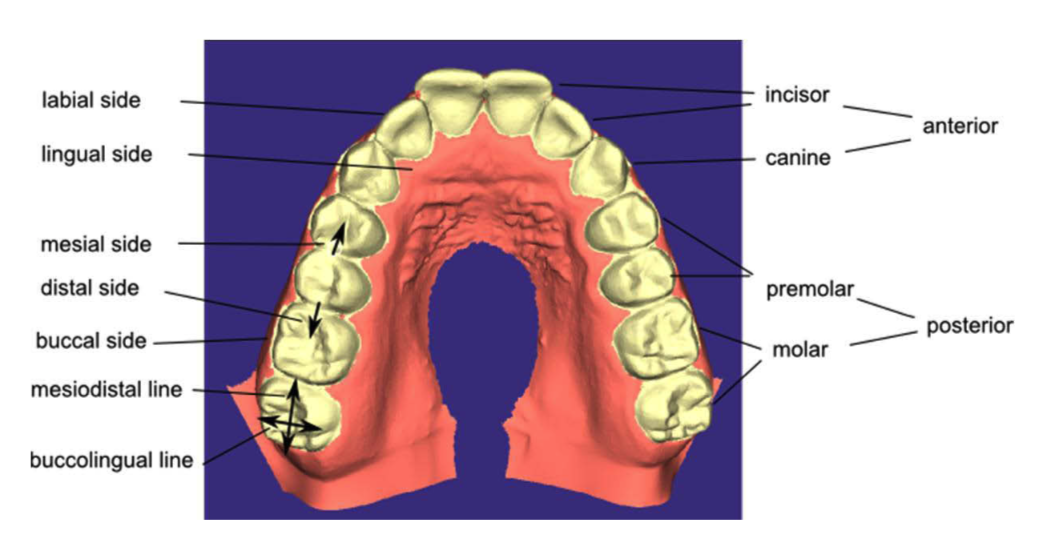
\includegraphics[width=1\linewidth]{images/dental_parts.png}
\caption{Анатомия зубов}
\label{fig:dental_parts}
\end{figure}

% ls | grep -e "^[0-9]" | while read dir; do ls $dir | nl | tail -n1; done

\subsubsection{Размер выборки}

В выборке присутствуют 28 типов зубов (все, кроме третьих моляров - зубов мудрости), для каждого типа зуба имеется от 124 до 150 экземпляров. Все экземпляры представлены в виде трехмерных сеток (перед началом работы основного алгоритма мы переводим их в облака точек, путем отбрасывания ребер). Примеры экземпляров из выборки можно увидеть на  изображениях:


\begin{figure}[h]
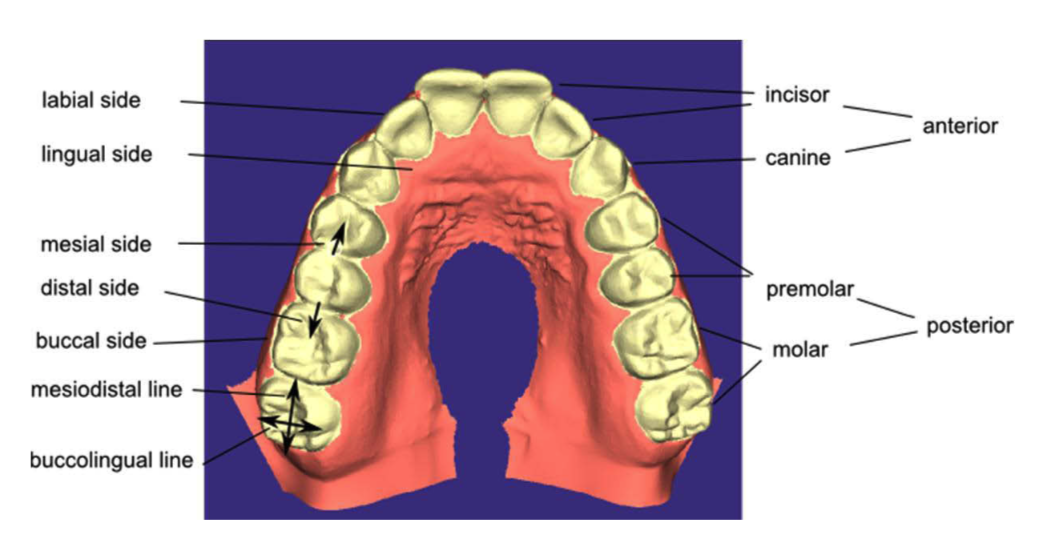
\includegraphics[width=1\linewidth]{images/dental_parts.png}
\caption{Анатомия зубов}
\label{fig:tooth_1}
\end{figure}


\begin{figure}[h]
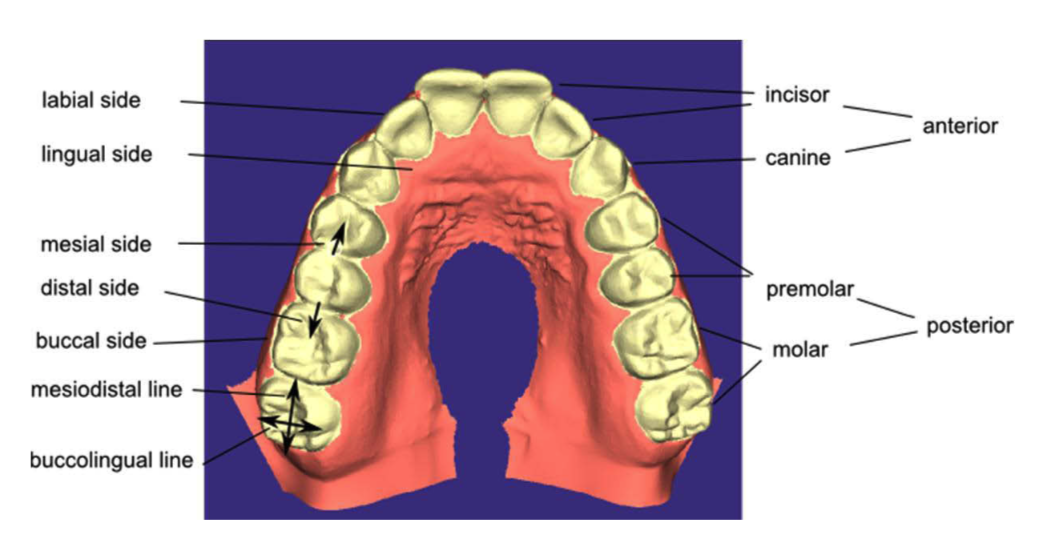
\includegraphics[width=1\linewidth]{images/dental_parts.png}
\caption{Анатомия зубов}
\label{fig:tooth_2}
\end{figure}


\begin{figure}[h]
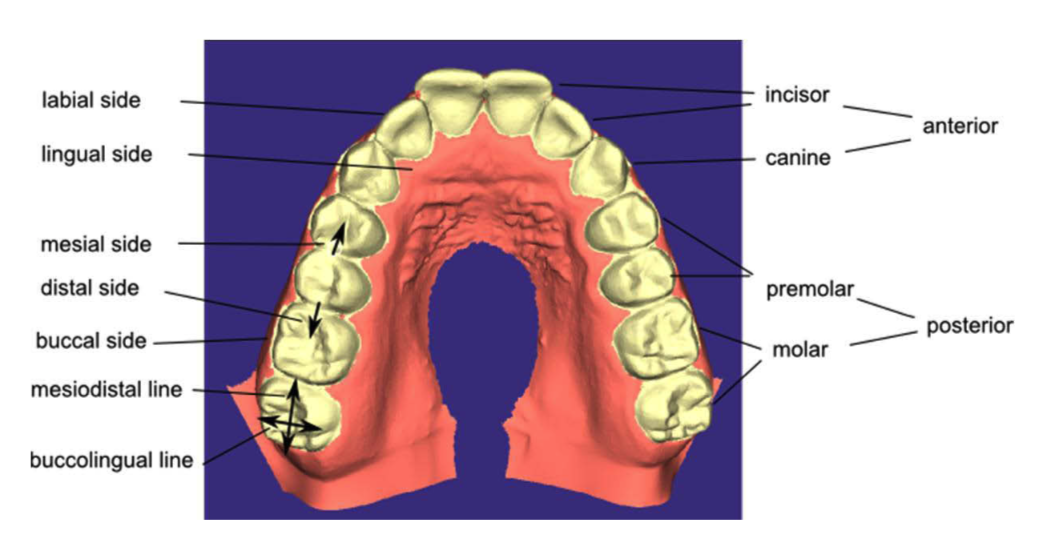
\includegraphics[width=1\linewidth]{images/dental_parts.png}
\caption{Анатомия зубов}
\label{fig:tooth_3}
\end{figure}
\section{Метрики сравнения облаков точек} \label{section:metrics-comparation}

\subsection{Проблема сравнения облаков точек}
% УВЕЛИЧЕНИЕ ОБЪЕМА!! SSIMD

Работа с облаками точек привносит ряд проблем в алгоритмы для их обработки и принципиально отличается от работы с двухмерными изображнениями. К примеру, в отличиии от двухмерных изображений, облака точек не имеют жесткой \textit{решетчатой структуры (grid-like structure)}, что приводит к невозможности использования многих алгоритмов из области обработки двухмерных ихображений при решении данной проблемы. Другой, не менее важной проблемой, является проблема упорядочивания самих точек в облаке. В общем случае, никакого порядка точек не существует, что создает инвариант перстановки (permutation invariant). То есть, в случае задания порядка точек в облаке, два облака с разными упорядочиваниями будут представлять абсолютно один и тот же трехмерный объект.

Вышеперечисленные проблемы сильно усложняют процесс сравнения двух облаков точек, который необходим для вычисления потерь алгоритма при восстановлении формы объектов, и приводят к необходимости выработки метрики, инвариантной к перестановкам порядка точек в облаке.


\subsection{Метрики сравнения облаков точек}

Одной из наиболее известных метрик для вычисления расстояния между компактными подмножествами метрического пространства является \textit{метрика Хаусдорфа}:

\[
	d_{H}(X,\;Y)=\max \left\{\sup\limits_{{x\in X}}\inf\limits_{{y\in Y}}|xy|,\;\sup\limits_{{y\in Y}}\inf\limits_{{x\in X}}|xy|\right\}
\]

Однако она является крайне неусточивой к небольшим выбросам во множествах.

% УВЕЛИЧЕНИЕ ОБЪЕМА!! привести пример
% http://dfgm.math.msu.su/files/ivanov-tuzhilin/2014-2015/METRGEOM2014-1.pdf
% привести пример

В работах \cite{metrics-source}, \cite{lrgm-cloud} были предложены две метрики: \textit{CD расстояние, (Расстояние Чамфера, Chamfer distance, CD)} и \textit{EMD расстояние (Earth Mover’s distance, EMD)}.

\subsubsection{CD расстояние}

Пусть \(S_{1}, S_{2} \subset \R^3\), тогда CD расстояние между ними определяется как:

\[
	d_{CD}(S_{1}, S_{2}) = \sum\limits_{x \in S_{1}} \min\limits_{y \in S_{2}} \norm{x - y}_{2}^{2} + \sum\limits_{x \in S_{1}} \min\limits_{y \in S_{2}} \norm{x - y}_{2}^{2}
\]

\medskip
Строго говоря CD расстояние не является метрикой, так-как не выполняется неравенство треугольника. Вычисление данной метрики для каждой пары точек проихсодит независимо, в связи с чем данная задача может быть эффективно распараллелена и скорость вычисления данной функции кратно увеличится. Также операции поиска ближайшего соседа могут быть существенно ускорены путем использования различных пространственных структура данных, таких как \textit{KD-деревья (KD-tree)}. 

% УВЕЛИЧЕНИЕ ОБЪЕМА!! В самом деле метрика + картинка
% УВЕЛИЧЕНИЕ ОБЪЕМА!! OpenCL
\subsubsection{EMD расстояние}

Рассмотрим множества \(S_{1}, S_{2} \subset \R^3\) одинакового размера \(s = \abs{S_{1}} = \abs{S_{2}}\). Тогда EMD расстояние между ними определяется как:

\[
	d_{EMD}(S_{1}, S_{2}) = \min\limits_{\phi:S_{1} \mapsto S_{2}} \sum\limits_{x \in S_{1}} \norm{x - \phi(x)}_{2}
\] где отображение \(\phi:S_{1} \mapsto S_{2}\) является биекцией.


Стоит отметить, что нахождение EMD расстояния аналогично решению задачи о назначениях \cite{assignment-task-1}, \cite{assignment-task-2}, которая решается \textit{Венгерским алгоритмом}\cite{hungarian-alg} за полиномиальное время (в худшем случае $O(n^4)$). Разумеется, на практике, точное вычисление EMD будет крайне ресурсозатратным, особенно для таких объектов как трехмерные изображения. В связи с чем, авторы статьи \cite{metrics-source} предлагают использовать аппроксимацию, которая позволяет более быстро вычислять ответ, пусть и с небольшими неточностями. Необходимо отметить, что данный метод работает для облаков точек с одинаковыми количествами точек.

% УВЕЛИЧЕНИЕ ОБЪЕМА!! Ухудшение из-за биекции
\bigskip
В результате, данные метрики обладают следующими свойствами:
\begin{enumerate}
\item Диффернцируемость относительно координат точек сравниваемых множеств
\item Устойчивость к малым выборсам
\item Относительная вычислительная эффективность для CD расстояния и для EMD аппроксимации
\end{enumerate}



В данной работе, при сравнении облаков точек, мы будем использовать CD расстояние, как более простое, более эффективное в реализации, интуитивно понятное и умеющее работать с облаками точек, состоящих из разных количеств точек.


\section{Метрики оценки генеративных моделей для трехмерных данных} \label{section:metrics-evaluation}


\section{Описание алгоритма} \label{section:algorithm}
\section{Результаты} \label{section:results}

В целом, алгоритм показал себя хорошо: на некоторах типов зубов показатели COV метрики достигали значений 0.9. Что при столь малом размере выборки является очень хорошим результатом. Для избеганий зависимости от разбиений выборки на тестовую и обучающую части была использована кросс-валиадация, с коэффициентом разбиения 10.

\subsection{Время работы}

Сам алгоритм на компьютере MacBook Pro(2015) с процессором 2,7 GHz Intel Core i5 при размере выборки в 150 элементов работает меньше чем за секунду. Во многом, такая скорость была достигнута за счет использования KD-деревьев для расчета CD-расстояния (см. \ref{section:metrics-comparation}).



Тем не менее, расчет метрик COV и MMD для оценивания качества сгенерированных объектов ...

\subsection{Метрики}

\subsection{Примеры данных}
На рисунках представлены результаты генерации новых зубов.
\section{Заключение} \label{section:conclusion}
\begin{thebibliography}{00}

% \bibitem{poz:diffgeom} Позняк Э.Г., Шикин Е.В.
% \emph{Дифференциальная геометрия: первое знакомство}. Москва, изд-во МГУ, 1990.


\bibitem{DLB} Ian Goodfellow and Yoshua Bengio and Aaron Courville
\emph{Deep Learning} MIT Press, 2016


\bibitem{deng-yu} Deng, L.; Yu, D. 
\emph{Deep Learning: Methods and Applications}
// Foundations and Trends in Signal Processing, 2014 1-199

\bibitem{peng-3d} Peng, Xingchao; Sun, Baochen; Ali, Karim; Saenko, Kate Saenko
\emph{Learning Deep Object Detectors from 3D Models} University of Massachusetts Lowell, 2015

\bibitem{Shrivastava-gap-real} Shrivastava, Ashish; Pfister, Tomas; Tuzel, Oncel; Susskind, Josh; Wang, Wenda; Webb, Russ 
\emph{Learning from Simulated and Unsupervised Images through Adversarial Training} arxiv.org, 2017

\bibitem{sanchez-at-glance} Sanchez, Cassie
\emph{At a Glance: Generative Models \& Synthetic Data} September 2017.

\bibitem{gan-1} Ian J. Goodfellow, Jean Pouget-Abadie, Mehdi Mirza, Bing Xu, David Warde-Farley, Sherjil Ozair, Aaron Courville, Yoshua Bengio
\emph{Generative Adversarial Networks} 2014

\bibitem{kumar} Y. Kumar, R. Janardan, and B. Larson, 
\emph{Automatic feature identification in dental meshes} Computer-Aided Design and Applications, vol. 9, no. 6, pp. 747–769, 2012.

\bibitem{gan-super} Christian Ledig, Lucas Theis, Ferenc Huszar, Jose Caballero, Andrew Cunningham, Alejandro Acosta, Andrew Aitken, Alykhan Tejani, Johannes Totz, Zehan Wang, Wenzhe Shi
\emph{Photo-Realistic Single Image Super-Resolution Using a Generative Adversarial Network} 2017

\bibitem{pu-net} Lequan Yu, Xianzhi Li, Chi-Wing Fu, Daniel Cohen-Or, Pheng-Ann Heng
\emph{PU-Net: Point Cloud Upsampling Network} The Chinese University of Hong Kong, Tel Aviv University, Shenzhen Institutes of Advanced Technology, Chinese Academy of Sciences, 2018

\bibitem{point-grid} Truc Le, Ye Duan
\emph{PointGrid: A Deep Network for 3D Shape Understanding} University of Missouri, 2018

\bibitem{point-net-plus} Charles R. Qi Li Yi Hao Su Leonidas J. Guibas
\emph{PointNet++: Deep Hierarchical Feature Learning on Point Sets in a Metric Space} Stanford University, 2017

\bibitem{octree-based} Peng-Shuai Wang, Yang Liu, Yu-Xiao Guo, Chun-Yu Sun, Xin Tong
\emph{O-CNN: Octree-based Convolutional Neural Networks for 3D Shape Analysis} 2017

\bibitem{spherical-conv-1} Huan Lei, Naveed Akhtar, Ajmal Mian
\emph{Spherical Convolutional Neural Network for 3D Point Clouds} University of Western Australia, 2018

\bibitem{spherical-cnn} Taco S. Cohen, Mario Geiger, Jonas Köhler, Max Welling
\emph{SPHERICAL CNNS} University of Amsterdam, 2018

\bibitem{3d-gan} Jiajun Wu, Chengkai Zhang, Tianfan Xue, William T. Freeman, Joshua B. Tenenbaum
\emph{Learning a Probabilistic Latent Space of Object Shapes via 3D Generative-Adversarial Modeling} 2017

\bibitem{3d-autoencoder} Andrew Brock, Theodore Lim, J.M. Ritchie, Nick Weston
\emph{Generative and Discriminative Voxel Modeling with Convolutional Neural Networks} 2016

\bibitem{adversarial-autoencoder} Maciej Zamorski, Maciej Zieba, Rafal Nowak, Wojciech Stokowiec and Tomasz Trzcinski
\emph{Adversarial Autoencoders for Generating 3D Point Cloud} 2018

\bibitem{seg-cloud} Lyne P. Tchapmi, Christopher B. Choy, Iro Armeni, JunYoung Gwak, Silvio Savarese
\emph{SEGCloud: Semantic Segmentation of 3D Point Clouds} 2017

\bibitem{lrgm-cloud} Panos Achlioptas, Olga Diamanti, Ioannis Mitliagkas, and Leonidas J Guibas.
\emph{Learning Representations and Generative Models For 3D Point Clouds} Proceedings
of the 35th International Conference on Machine Learning 2018

\bibitem{metrics-source} Haoqiang Fan, Hao Su, Leonidas Guibas
\emph{A Point Set Generation Network for 3D Object Reconstruction from a Single Image} arXiv e-prints 2016

\bibitem{stat-shape-1} Alan Brunton, Augusto Salazar, Timo Bolkart, Stefanie Wuhrer
\emph{Statistical Shape Spaces for 3D Data: A Review} Chi Hau Chen. Handbook of Pattern Recognition and Computer Vision, 5th Edition, 2016, 978-981-4656-52-8. 

\bibitem{stat-shape-2} Alan Brunton, Augusto Salazar, Timo Bolkart, Stefanie Wuhrer
\emph{Review of Statistical Shape Spaces for 3D Data with Comparative Analysis for Human Faces}

\bibitem{bishop} Christopher M. Bishop
\emph{Pattern Recognition and Machine Learning} Information Science and Statistics, 2006


\bibitem{assignment-task-1} Хемди А. Таха.
\emph{Введение в исследование операций} 7-е издание. Пер. с англ. — М.: Издательский дом «Вильямс», 2005.

\bibitem{assignment-task-2} Вагнер Г.
\emph{Основы исследования операций} Пер. с англ. — М.: Издательство «Мир», 1972.. — Т. 1.

\bibitem{hungarian-alg} Harold W. Kuhn
\emph{Variants of the Hungarian method for assignment problems} Naval Research Logistics Quarterly, 3: 253—258, 1956

\bibitem{python:doc} Python v3.5 documentation
[HTML] (http://docs.python.org/3.5).

\bibitem{python:lutz} Лутц М.
\emph{Изучаем Python, 4-е издание.} – Пер. с англ. – СПб.: Символ-Плюс, 2011.

\bibitem{wahba} Wahba, G. 
\emph{Problem 65–1: A Least Squares Estimate of Spacecraft Attitude}, SIAM Review, 1965, 7(3), 409


\bibitem{icp-main} P.J. Besl, N.D. McKay.
\emph{A method for registration of 3D shapes} IEEE Transactions on Pattern Analysis and Machine Intellinegce 14 (1992) 239– 254.

\bibitem{icp-2} B. K. P. Horn 
\emph{Closed-form solution of absolute orientation using unit quaternions} J. Opt. Soc. Amer. Avol. 4, no. 4, pp. 629-642, Apr. 1987.
\end{thebibliography}
\end{document}